\chapter{Estimating pose and structure} \label{ch:estimating-pose-and-structure}
\begin{figure}[htb]
    \centering
    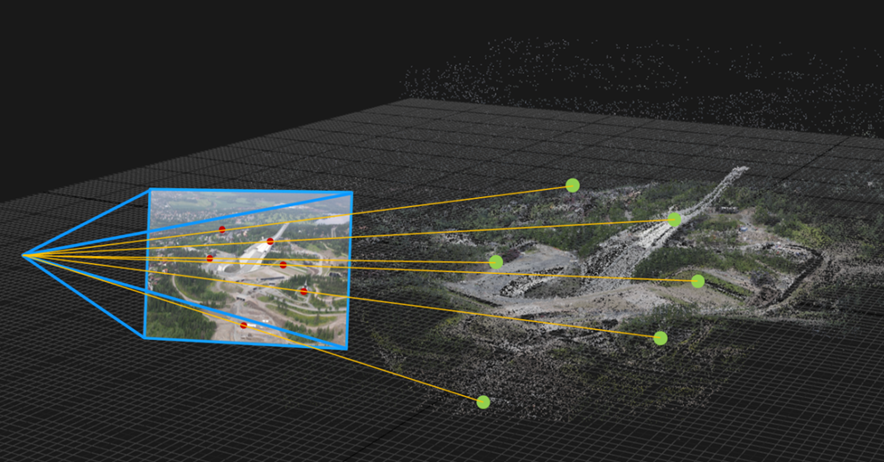
\includegraphics[width=\columnwidth]{figures/moba.png}
    \caption{An example of estimating pose from correspondences between pixel points and 3D points in a map.
    }
    \label{fig:moba}
\end{figure}

This chapter gives a brief introduction to how we can estimate pose and structure from images, based on the principles we have covered in the previous chapters.

Pose estimation using cameras is also sometimes called \emph{motion estimation} or \emph{localisation}, and is usually estimated relative to known structure, as illustrated in Figure~\ref{fig:moba}.
The \emph{structure} is here a representation of the 3D structure in the scene, which is also sometimes called a \emph{map}.
When we know the relative poses between two or more cameras, we can estimate the structure by triangulating correspondences between the cameras.

When neither pose nor structure is known a priori, we typically need to \emph{initialise} a map based on relative pose estimates between camera images.
We can then estimate new poses relative to this map, and continue extending the map while exploring the scene.
This procedure is often called \emph{simultaneous localisation and mapping (SLAM)}, and performing SLAM with images is often called \emph{Visual SLAM (VSLAM)}.

A major problem with monocular vision is that scale in the world cannot be observed without prior knowledge. 
Monocular VSLAM will therefore drift in scale over time, and this results in a major contribution to the overall error. 
But as pointed out in \cite{Engel2014LSD-SLAM:SLAM}, an interesting paradox is that its inherent scale-ambiguity is also a major benefit, since monocular vision can seamlessly operate in vastly differently scaled environments, such as switching from a small-scale door handle to the large-scale environment just outside.

Adding more sensors, such as another camera with known baseline, active range sensors or an inertial navigation system, can enable us to recover metric scale, as well as the horizontal plane, and even the geographical pose.

\section{Problem formulations}
It is common to formulate pose estimation problems as either \emph{direct} or \emph{indirect}, and structure estimation problems as either \emph{dense} or \emph{sparse} \cite{Engel2018}.

\emph{Indirect methods} first extract an intermediate geometrical representation of the scene, such as keypoint correspondences or optical flow vectors, and use these to optimise a \emph{geometric error}.
Because these methods are based on some kind of feature extraction step, they are also often called \emph{feature-based methods}.
Indirect methods provide robustness to photometric and geometric distortions, but come at the price of higher computational cost and are dependent on the feature extraction step to work.

\emph{Direct methods} skip the feature extraction step, and use the image intensity values directly to optimise a \emph{photometric error}.
Direct methods do not require that geometrical primitives are recognisable by themselves, but can sample across all parts of the image.
This makes direct methods more robust to effects such as motion blur and better suited in environments that are sparsely textured, but they are vulnerable to photometric and geometric distortions.

\emph{Sparse methods} reconstruct and use only a selected set of independent points in the scene, while \emph{dense methods} attempt to reconstruct and use a 3D map for all the pixels in the images.
An important difference between the sparse and dense methods is that, while the sparse methods map independent points with no notion of neighbourhoods, the dense methods typically add a geometric prior, assuming that the structure is locally smooth.
Because of the resulting correlated structure in the dense maps, it is difficult to optimise pose and dense structure jointly in real-time.

The most widely used formulation is the sparse indirect formulation, which is used in methods such as PTAM \cite{Klein2007ParallelWorkspaces} and ORB-SLAM \cite{Mur-Artal2015ORB-SLAM:System}.
The sparse direct formulation is used in DSO \cite{Engel2018}, while the dense direct formulation is used in DTAM \cite{Newcombe2011DTAM:Real-time} and LSD-SLAM \cite{Engel2014LSD-SLAM:SLAM}.
SVO \cite{Forster2014SVO:Odometry} uses a hybrid formulation, where the direct formulation is used for initial alignment and to obtain correspondences, while the indirect formulation is used for joint model optimisation.

We will in the following sections take a closer look at how we can express and solve some of these problems.


\section{Indirect methods}
We will here consider sparse, indirect methods based on point correspondence measurements between images.
Given correspondences $\vecu \leftrightarrow \vecx^w$ between pixels and points in the world frame (defined by the map), these methods minimise the \emph{geometric error}, which for each correspondence can be expressed as
\begin{equation}
  e_g(\matT_{wc}, \vecx^w) = \pi_p(\matT_{wc}^{-1} \cdot \vecx^w) - \vecu.
\end{equation}
Here, $\pi_p$ is the projection function for the perspective camera given in \eqref{eq:projection-function} and $\matT_{wc}$ is the pose of the camera in the world frame.
The geometric error measures the difference between the predicted pixel position, given the current hypotheses for the pose $\matT_{wc}$ and the point $\vecx^w$, and the measured pixel correspondence.
It is therefore also often called the \emph{reprojection error}.
Estimating poses and structure based on the geometric error is often called \emph{bundle adjustment} \cite{Triggs2000BundleSynthesis}.

The following sections will discuss how we can estimate pose, structure and both, based on minimising the geometric error.

\subsection{Estimating pose with known structure}
Assume that the world points $\vecx^w_j$ are known, and we are given the correspondences $\vecu_j \leftrightarrow \vecx^w_j$, with measurement noise $\matSigma_j$.

A suitable initial estimate for the pose $\matT_{wc}$ can be found by applying a fast \emph{perspective-n-point (PnP)} algorithm, such as P3P \cite{Kneip2011AOrientation}.
Estimating the camera pose from known 3D points by minimising the geometric error is sometimes called \emph{motion-only bundle adjustment}.
Assuming that the camera is calibrated, we can pre-calibrate the measurements to normalised image coordinates with \eqref{eq:normalised-from-pixel}.
This gives us the measurement prediction function
\begin{equation}
  h_j(\matT_{wc}) = \pi_n(\matT_{wc}^{-1} \cdot \vecx^w_j),
\end{equation}
where $\pi_n$ is the projection function to normalised image coordinates in \eqref{eq:normalised-projection-function}.
The measurement error function is the geometric error
\begin{equation}
  e_j(\matT_{wc}) = \pi_n(\matT_{wc}^{-1} \cdot \vecx^w_j) - \vecx_{n \; j}.
\end{equation}

The Jacobian of the measurement prediction function is given by (omitting the index $j$ for brevity)
\begin{subequations} \label{eq:ba-pose-jacobian}
\begin{align}
  \jac{h}{\matT_{wc}} &= \jac{\pi_n(\matT_{wc}^{-1} \cdot \vecx^w)}{\matT_{wc}^{-1} \cdot \vecx^w} \jac{\matT_{wc}^{-1} \cdot \vecx^w}{\matT_{wc}^{-1}} \jac{\matT_{wc}^{-1}}{\matT_{wc}}\\
  &= \jac{\pi_n(\vecx^c)}{\vecx^c} \jac{\matT_{wc}^{-1} \cdot \vecx^w}{\matT_{wc}^{-1}} \jac{\matT_{wc}^{-1}}{\matT_{wc}}\\
  &= \frac{1}{z^c}
  \begin{bmatrix}
  1 & 0 & -x^c/z^c\\
  0 & 1 & -y^c/z^c
  \end{bmatrix}
  \begin{bmatrix}
    \matR_{wc}\trans & -\matR_{wc}\trans \skewsymm{\vecx^w}
  \end{bmatrix}
  \cdot
  -\begin{bmatrix}
    \matR_{wc} & \skewsymm{\vect^w_{wc}} \matR_{wc}\\
    \matr{0} & \matR_{wc}
  \end{bmatrix}\\
  &= d
  \begin{bmatrix}
  1 & 0 & -x_n\\
  0 & 1 & -y_n
  \end{bmatrix}
  \begin{bmatrix}
  -\matI & \skewsymm{\vecx^c}
  \end{bmatrix}\\
  &=
  \begin{bmatrix}
    -d & 0 & dx_n & x_n y_n & -1-x^2_n & y_n\\
    0 & -d & dy_n & 1 + y^2_n & -x_n y_n & -x_n
  \end{bmatrix},
\end{align}
\end{subequations}
where $\vecx^c = \matT_{wc}^{-1} \cdot \vecx^w$ is the point in camera frame, and $d = 1/z^c$ is the inverse depth.

By propagating the noise to the normalised image plane, we get the linearised weighted least squares problem
\begin{align}
  \vecxi^\ast &= \argmin_{\vecxi} \sum^n_{j=1} \norm{ \matA_j \vecxi - \vecb_j}^2\\
  &= \argmin_{\vecxi} \norm{ \matA \vecxi - \vecb}^2,
\end{align}
where
\begin{align}
  \matA_j &= \matSigma^{-1/2}_{n \; j} \jac{h_j}{\matT_{wc}}\\
  \vecb_j &= \matSigma^{-1/2}_{n \; j} (\vecx_{n \; j} - h_j(\matT_{wc})),
\end{align}
and
\begin{equation}
  \matA =  
  \begin{bmatrix}
    \matA_1\\
    \vdots\\
    \matA_n
  \end{bmatrix}
  \qquad
  \vecb =  
  \begin{bmatrix}
    \vecb_1\\
    \vdots\\
    \vecb_n
  \end{bmatrix}.
\end{equation}

This lets us compute the MAP estimate $\hat{\matT}_{wc}$ with Gauss-Newton or Levenberg-Marquardt.

\subsection{Estimating structure with known poses}
Assume that we know the poses of the two or more cameras $\{ \matT_{wc_i}\}$, and we are given the correspondences $\vecu^i_j \leftrightarrow \vecx^w_j$, with measurement noise $\matSigma_{ij}$.

A suitable initial estimate for the structure $\{ \vecx^w_j \}$ can be found by for example triangulating the points linearly by minimising algebraic error \cite{Hartley2004MultipleVision}.
Estimating the structure from known camera poses by minimising the geometric error is sometimes called \emph{structure-only bundle adjustment}.
Assuming that the cameras are calibrated, we can pre-calibrate the measurements to normalised image coordinates with \eqref{eq:normalised-from-pixel}.
This gives us the measurement prediction function
\begin{equation}
  h_{ij}(\vecx^w_j) = \pi_n(\matT_{wc_i}^{-1} \cdot \vecx^w_j),
\end{equation}
where $\pi_n$ is the projection function to normalised image coordinates in \eqref{eq:normalised-projection-function}.
The measurement error function is the geometric error
\begin{equation}
  e_{ij}(\vecx^w_j) = \pi_n(\matT_{wc_i}^{-1} \cdot \vecx^w_j) - \vecx_{n \; j}^i.
\end{equation}

The Jacobian of the measurement prediction function is given by (omitting the indexes $i$ and $j$ for brevity)
\begin{subequations} \label{eq:ba-structure-jacobian}
\begin{align}
  \jac{h}{\vecx^w} &= \jac{\pi_n(\matT_{wc}^{-1} \cdot \vecx^w)}{\matT_{wc}^{-1} \cdot \vecx^w} \jac{\matT_{wc}^{-1} \cdot \vecx^w}{\vecx^w}\\
  &= \jac{\pi_n(\vecx^c)}{\vecx^c}  \jac{\matT_{wc}^{-1} \cdot \vecx^w}{\vecx^w}\\
  &= \frac{1}{z^c}
  \begin{bmatrix}
  1 & 0 & -x^c/z^c\\
  0 & 1 & -y^c/z^c
  \end{bmatrix}
  \matR_{wc}\trans\\
  &= d
  \begin{bmatrix}
  1 & 0 & -x_n\\
  0 & 1 & -y_n
  \end{bmatrix}
  \matR_{wc}\trans,
\end{align}
\end{subequations}
where $\vecx^c = \matT_{wc}^{-1} \cdot \vecx^w$ is the point in camera frame, and $d = 1/z^c$ is the inverse depth.

By propagating the noise to the normalised image plane, we get the linearised weighted least squares problem
\begin{align}
  \delta\vecx^\ast &= \argmin_{\delta\vecx} \sum^k_{i=1} \sum^n_{j=1} \norm{ \matA_{ij} \delta\vecx_j - \vecb_{ij}}^2\\
  &= \argmin_{\delta\vecx} \norm{ \matA \delta\vecx - \vecb}^2,
\end{align}
where
\begin{align}
  \matA_{ij} &= \matSigma^{-1/2}_{n \; {ij}} \jac{h_{ij}}{\vecx^w_j}\\
  \vecb_{ij} &= \matSigma^{-1/2}_{n \; {ij}} (\vecx_{n \; j}^i - h_{ij}(\vecx^w_j)),
\end{align}
and

\begin{equation}
  \matA =  
  \begin{bmatrix}
    \matA_{11} & & \\
    & \ddots & \\
    & & \matA_{1n}\\
    & \vdots &\\
    \matA_{k1} & & \\
    & \ddots & \\
    & & \matA_{kn}
  \end{bmatrix}
  \qquad  
  \delta\vecx =
  \begin{bmatrix}
    \delta\vecx_1\\
    \vdots\\
    \delta\vecx_n
  \end{bmatrix}
  \qquad
  \vecb =  
  \begin{bmatrix}
    \vecb_{11}\\
    \vdots\\
    \vecb_{1n}\\
    \vdots\\
    \vecb_{k1}\\
    \vdots\\
    \vecb_{kn}
  \end{bmatrix}.
\end{equation}

This lets us compute the MAP estimates $\{\hat{\vecx}^w_j\}$ with Gauss-Newton or Levenberg-Marquardt.


\subsection{Estimating pose and structure}
In this situation we do not know either the camera poses $\{ \matT_{wc_i}\}$ nor the world points $\{ \vecx^w_j \}$.
We are just given the correspondences $\vecu^i_j \leftrightarrow \vecx^w_j$, with measurement noise $\matSigma_{ij}$.

A suitable initial estimate can be found by first applying pairwise two-view relative pose estimation, based on estimating the essential matrix $\matE$ using the 5-point algorithm \cite{Nister2004AnProblem}, and decomposing it to obtain the relative pose \cite{Hartley2004MultipleVision}.
Estimating the both pose and structure by minimising the geometric error is sometimes called \emph{full bundle adjustment}.
Assuming that the cameras are calibrated, we can pre-calibrate the measurements to normalised image coordinates with \eqref{eq:normalised-from-pixel}.
This gives us the measurement prediction function
\begin{equation}
  h_{ij}(\matT_{wc_i}, \vecx^w_j) = \pi_n(\matT_{wc_i}^{-1} \cdot \vecx^w_j),
\end{equation}
where $\pi_n$ is the projection function to normalised image coordinates in \eqref{eq:normalised-projection-function}.
The measurement error function is the geometric error
\begin{equation}
  e_{ij}(\matT_{wc_i}, \vecx^w_j) = \pi_n(\matT_{wc_i}^{-1} \cdot \vecx^w_j) - \vecx_{n \; j}^i.
\end{equation}

Since the measurement function is a function of two variables, we linearise it at the current state estimates as
\begin{subequations}
\begin{align}
    h_{ij}(\matT_{wc_i}, \vecx^w_j) &= h_{ij}(\hat{\matT}_{wc_i} \oplus \vecxi_i, \hat{\vecx}^w_j + \delta\vecx_j) \\
    &\approx h_{ij}(\hat{\matT}_{wc_i}, \hat{\vecx}^w_j) + \jac{h_{ij}}{\hat{\matT}_{wc_i}}\vecxi_i + \jac{h_{ij}}{\hat{\vecx}^w_j}\delta\vecx_j,
\end{align}
\end{subequations}
The Jacobians are given in \eqref{eq:ba-pose-jacobian} and \eqref{eq:ba-structure-jacobian}.

By propagating the noise to the normalised image plane, we get the linearised weighted least squares problem
\begin{align}
  \ubar{\vectau}^\ast &= \argmin_{\ubar{\vectau}} \sum^k_{i=1} \sum^n_{j=1} \norm{ \matP_{ij} \vecxi_i + \matS_{ij} \delta\vecx_j - \vecb_{ij}}^2\\
  &= \argmin_{\ubar{\vectau}} \norm{ \matA \ubar{\vectau} - \vecb}^2,
\end{align}
where
\begin{align}
  \matP_{ij} &= \matSigma^{-1/2}_{n \; {ij}} \jac{h_{ij}}{\matT_{wc_i}}\\
  \matS_{ij} &= \matSigma^{-1/2}_{n \; {ij}} \jac{h_{ij}}{\vecx^w_j}\\
  \vecb_{ij} &= \matSigma^{-1/2}_{n \; {ij}} (\vecx_{n \; j}^i - h_{ij}(\matT_{wc_i}, \vecx^w_j)),
\end{align}
and
\begin{equation} \label{eq:ba-matrices}
  \matA =  
  \begin{bmatrix}
    \matP_{11} &  &  & \matS_{11} & & \\
    \vdots & & & & \ddots & \\
    \matP_{1n} & & & & &\matS_{1n}\\
    & \ddots &  & & \vdots &\\
    & & \matP_{k1} & \matS_{k1} & & \\
    & & \vdots & & \ddots & \\
    & & \matP_{kn}& & &\matS_{kn}
  \end{bmatrix}
  \qquad  
  \ubar{\vectau} =
  \begin{bmatrix}
    \vecxi_1\\
    \vdots\\
    \vecxi_k\\
    \delta\vecx_1\\
    \vdots\\
    \delta\vecx_n
  \end{bmatrix}
  \qquad
  \vecb =  
  \begin{bmatrix}
    \vecb_{11}\\
    \vdots\\
    \vecb_{1n}\\
    \vdots\\
    \vecb_{k1}\\
    \vdots\\
    \vecb_{kn}
  \end{bmatrix}.
\end{equation}

The linear least squares problem in \eqref{eq:ba-matrices} is not uniquely determined and has a singular approximation to the Hessian.
This is because the global frame and scale is not defined, so we can apply any similarity transform to the camera poses without affecting the objective function.
This is sometimes called \emph{gauge freedom}.
We fix this by adding priors on at least one pose, defining the global frame, and at least one point, defining the global scale.

This lets us compute the MAP estimates $\{\hat{\matT}_{wc_i}\}$ and $\{\hat{\vecx}^w_j\}$ with Gauss-Newton or Levenberg-Marquardt.


\section{Direct methods} \label{sec:direct-methods}
We will here consider direct methods that optimise structure separately from pose.

Consider two images $I_a(\vecu)$ and $I_b(\vecu)$.
Given the relative pose $\matT_{ab}$ between the two cameras $a$ and $b$, we can define the \emph{warp function} \cite{Baker2004Lucas-KanadeFramework}
\begin{equation}
  \vecu^a = w(\vecu^b, z^b, \matT_{ab}) = \pi_p(\matT_{ab} \cdot  \pi_p^{-1}(\vecu^b, z^b)),
\end{equation}
that maps a pixel $\vecu^b$ in image $I_b$ to a pixel $\vecu_a$ in image $I_a$.
This lets us define the \emph{photometric error} between these two images at a given pixel as
\begin{equation} \label{eq:photometric-error}
  e_p(\vecu^b, z^b, \matT_{ab}) = I_a(w(\vecu^b, z^b, \matT_{ab})) - I_b(\vecu^b).
\end{equation}

Direct methods typically represent structure as a sparse or dense depth map for pixels rather than 3D points.
The depth is typically represented as the \emph{inverse depth} $d = z^{-1}$, because the inverse depth parameterisation is better suited when we want to model the uncertainty in depth using a Gaussian noise model \cite{Civera2012InverseParametrization}.
Depth can be estimated by collecting small-baseline measurements over time, letting the uncertainty in depth fall below a threshold before using it for pose estimation \cite{Engel2013Semi-denseCamera, Engel2014LSD-SLAM:SLAM, Forster2014SVO:Odometry}.

If we know the pose $\matT_{ab}$ between the two images, we can exploit the epipolar geometry to search for good matches that minimises \eqref{eq:photometric-error} over a relevant interval of depths, guided by the current depth uncertainty (Section~\ref{sec:epipolar-geometry}).
Since
\begin{equation}
  z^a \matK^{-1}_a \breve{\vecu}^a = z^b \matR_{ab} \matK^{-1}_b \breve{\vecu}^b + \vect^a_{ab},
\end{equation}
we can compute both depths by solving the linear least squares problem
\begin{equation}
  \vecz^\ast = \argmin_\vecz \norm{\matA\vecz - \vecb}^2,
\end{equation}
where
\begin{equation}
  \matA = 
  \begin{bmatrix}
    \matK^{-1}_a \breve{\vecu}^a & -\matR_{ab} \matK^{-1}_b \breve{\vecu}^b
  \end{bmatrix}
  \qquad
  \vecz = 
  \begin{bmatrix}
    z^a\\
    z^b
  \end{bmatrix}
  \qquad
  \vecb = \vect^a_{ab}.
\end{equation}

When interested in $z^j$ only, the law of sines applied on the epipolar plane gives us
\begin{equation}
  z^b = \frac{\norm{\matK_a^{-1} \breve{\vecu}^a \times \vect^a_{ab}}} {\norm{\matK_a^{-1} \breve{\vecu}^a \times \matR_{ab} \matK^{-1}_b \breve{\vecu}^b}}.
\end{equation}
We can avoid the computations of the norms by
\begin{equation}
  z^b = \frac{\veca\trans (\matK_a^{-1} \breve{\vecu}^a \times \vect^a_{ab})} {\veca\trans (\matK_a^{-1} \breve{\vecu}^a \times \matR_{ab} \matK^{-1}_b \breve{\vecu}^b)},
\end{equation}
where $\veca \in \bbR^3$ is a suitable vector that is not perpendicular to the epipolar plane, or parallel to any of the vectors in the cross products.

Assuming that the cameras are calibrated, we can pre-calibrate the measurements to normalised image coordinates with \eqref{eq:normalised-from-pixel}.
This results in the warp function
\begin{equation}
  w_n(\vecx^b_n, z^b, \matT_{ab})) = \pi_n(\matT_{ab} \cdot \pi_n^{-1}(\vecx^b_n, z^b)).
\end{equation}
Given the depths $\{z^b_i\}$ for normalise image coordinates $\{\vecx^b_{n \; i}\}$ and the images $I_a$ and $I_b$, we can estimate the pose $\matT_{ab}$ by defining the measurement prediction function for the pixel intensity in image $I_b$ as
\begin{equation}
  h_i(\matT_{ab}) = I_a(w_n(\vecx^b_{n \; i}, z^b_i, \matT_{ab})),
\end{equation}
and the measurement error function as
\begin{equation}
 e_i(\matT_{ab}) = I_a(w_n(\vecx^b_{n \; i}, z^b_i, \matT_{ab})) - I_b(\vecx^b_{n \; i}).
\end{equation}

The Jacobian of the measurement prediction function is given by (omitting the indexes $i$ for brevity)
\begin{subequations} \label{eq:direct-pose-jacobian}
\begin{align}
  \jac{h}{\matT_{ab}} &= \jac{I_a}{w_n(\vecx^b_n, z^b, \matT_{ab})} \jac{w_n(\vecx^b_n, z^b, \matT_{ab})}{\matT_{ab}}\\
  &= \jac{I_a}{\pi_n(\vecx^a)} \jac{\pi_n(\matT_{ab} \cdot \vecx^b)}{\matT_{ab} \cdot \vecx^b} \jac{\matT_{ab} \cdot \vecx^b}{\matT_{ab}}\\
  &= \jac{I_a}{\vecx^a_n} \jac{\pi_n(\vecx^a)}{\vecx^a} \jac{\matT_{ab} \cdot \vecx^b}{\matT_{ab}}\\
  &= \nabla I_a(\vecx^a_n) \;
   d
  \begin{bmatrix}
  1 & 0 & -x^a_n\\
  0 & 1 & -y^a_n
  \end{bmatrix}
  \begin{bmatrix}
    \matR_{ab} & -\matR_{ab} \skewsymm{\vecx^b}
  \end{bmatrix},
\end{align}
\end{subequations}
where $\nabla I_a(\vecx^a_n)$ is the image gradient at $\breve{\vecu}^a = \matK_a \breve{\vecx}^a_n$.

This lets us compute the MAP estimate $\hat{\matT}_{ab}$ with Gauss-Newton or Levenberg-Marquardt.

% \section{Structure from Motion and Visual SLAM} \label{sec:sfm-and-vslam}
% \begin{figure}[htb]
%     \centering
%     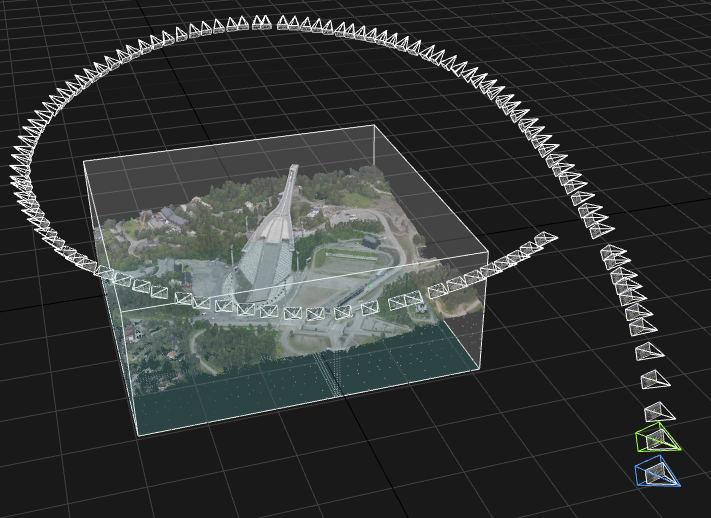
\includegraphics[width=0.75\columnwidth]{figures/holmenkollen-3d.png}
%     \caption{An example of structure from motion and 3D reconstruction based only on the images themselves.
%     }
%     \label{fig:sfm}
% \end{figure}
% Two different research fields in particular have been involved in studying methods for estimating motion and scene structure simultaneously using cameras, which is a difficult and highly nonlinear problem.

% The SLAM field within robotics have traditionally been using sequential filtering methods \cite{Thrun2002ProbabilisticRobotics} to estimate the real-time motion of robots and the position of landmarks, often in combination with other sensors.
% Traditional nonlinear filtering methods, such as the EKF\footnote{Extended Kalman Filter}, achieve fast estimation rates by updating just based on the current states, since previous states are marginalised out when new states are added.
% These methods also choose linearisation points for new states at the current time, and maintain these linearisations throughout the estimation.
% This will cause linearisation errors that accumulate over time, causing the solution to drift and the filter to become inconsistent.

% The structure from motion (SFM) field in computer vision has evolved from photogrammetry, and has traditionally focused their work on offline 3D reconstruction of the environment based on batch optimisation through \textit{bundle adjustment} \cite{Triggs2000BundleSynthesis}.
% Smoothing approaches such as this are generally more accurate than filtering, since they are able to relinearise past measurements.
% In addition, by keeping past states it is easy to add measurements with high latency and to perform loop closures when areas are revisited.
% The last 10 years or so has seen the bridging of the gap between these two fields, where the de-facto standard now is to formulate the mapping problem as a batch MAP estimation problem \cite{Strasdat2012VisualFilter, Cadena2016}, typically based on \emph{factor graphs}.

% \begin{figure}[htb]
%     \centering
%     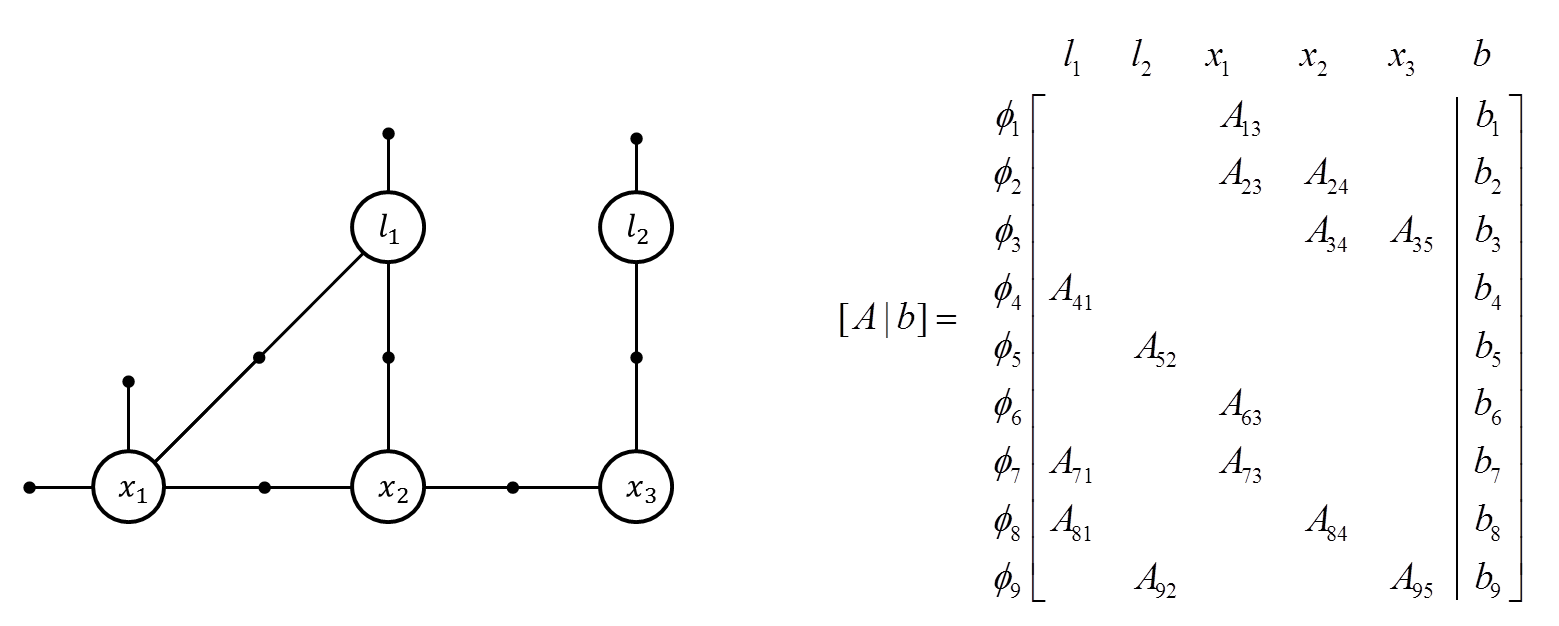
\includegraphics[width=\columnwidth]{figures/factor-graph-structure.png}
%     \caption{An example of a factor graph for a simple SLAM problem. 
%     On the left we see a visualisation of the factor graph.
%     Circles denote the state variable nodes for the poses $x_i$ and the landmark positions $l_j$. 
%     The black dots represent the factors corresponding to priors and measurements on the variables. 
%     The unary factors on $x_1$, $l_1$ and $l_2$ correspond to priors on these variables, while $x_1$ has an additional unary factor corresponding to a GPS measurement. 
%     The binary factors between poses represent odometry measurements, while the factors between poses and landmarks are bearing measurements.
%     The matrix to the right shows how the graph encodes the structure of the Jacobian $\matA$.
%     }
%     \label{fig:factor-graphs}
% \end{figure}
% A factor graph represents the estimation problem as a graphical model, and provides powerful tools for expressing and solving nonlinear estimation problems \cite{Dellaert2017}.
% It lets us specify constraints on state variables directly in a modular way, by specifying measurement prediction functions and Jacobians.
% The graph encodes dependencies directly, implicitly representing large sparse Jacobian matrices like \eqref{eq:ba-structure-jacobian}, by working only on the relevant blocks (Figure~\ref{fig:factor-graphs}).
% The estimation procedure is usually based on nonlinear least squares, as presented in Chapter~\ref{ch:nls}.

% It is customary to separate a SLAM system into two main components: the \emph{front end} and the \emph{back end} \cite{Cadena2016}.
% The front end extracts relevant data and data associations from raw sensor measurements, while the back end performs estimation and inference on data from the front end.
% Since the introduction of the ground breaking VSLAM system \emph{Parallel Tracking and Mapping} (PTAM) by Klein and Murray \cite{Klein2007ParallelWorkspaces}, VSLAM architectures are typically separated into a front end \emph{tracking} component, which estimates camera motion by tracking the scene structure using a map, and a back end \emph{mapping} component that builds the map based on observations.
% The key insight here was that these two components could be executed separately in different threads, allowing real-time pose estimation for each consecutive frame, while simultaneously updating and optimising the map at a lower rate on a selected set of spatially distributed \emph{keyframes}.

% In visual SLAM, the variables $X$ are often 3D camera poses and landmark positions.
% The factors between the pose variables and the landmark variables encode the errors in the predicted landmark projections for each camera using the current hypothesis $X^k$, compared to the actual measurements $Z$.
% The prior factors on camera poses and landmark positions encode the errors in the assumed state compared to the hypothesis.
% Given an appropriate motion model, for example, factors between camera poses can also be defined.
% In fact, by defining appropriate measurement prediction functions and Jacobians, any additional constraints between variables based on measurements from other sources, such as IMUs, GNSS, barometers and lidars \cite{Chiu2014}, can also be included in the optimisation as new factors.
% Additional variables such as calibration parameters can similarly be included by extending the measurement models.
% This is what makes the factor graph framework a powerful tool for VSLAM and data fusion in general.

% Factor graph implementations \cite{Kummerle2011G2o:Optimization, KuemmerleG2oSource, Dellaert2012FactorIntroduction, Dellaert2018GTSAMSource} provide \emph{full batch} solvers based on sparse linear algebra, that can be used in real time in the PTAM architecture.
% This can be combined with \emph{fixed-lag smoothers} \cite{Strasdat2011DoubleSLAM, Chiu2013}, that achieves constant estimation time by performing optimisation over a fixed window of states, while marginalising out the rest.
% There are also incremental solvers that efficiently update the solution given new data \cite{Kaess2012ISAM2:Tree}.
% Full (incremental) smoothing and (incremental) fixed-lag smoothing may also be combined in what is called \textit{concurrent smoothing and mapping} \cite{Kaess2012, Chiu2013}, and allows constant-time estimation with full batch optimisation over the same factor graph.
% Finally, there are also solvers that relax the assumption on Gaussian noise, and may perform full batch and incremental inference over non-parametric multimodal distributions \cite{Fourie2016, Fourie2017Multi-modalGraphs, incrementalinferencejl}. 
% This is especially interesting when data associations are uncertain, for example when you know you are close to a house, but not which of several possible houses in a given prior map.
% The multimodal factor graph framework makes it possible to perform inference over multiple hypotheses in this situation, enabling the back end to exploit more information than would otherwise be possible.

